\documentclass[12pt,fleqn]{article}\usepackage{../../common}
\begin{document}
Ders 11

Konumuz kesit seviyeleri (level sets). Bu alanda Sethian ve Osher otorite
say�l�yor, 80'li y�llarda yay�nlad�klar� makale ve kitaplarda konuyu etrafl�ca
i�lediler.

Elimizde bir e�ri var diyelim (altta resimde $t=0$ an�ndaki)

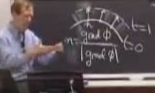
\includegraphics[width=20em]{2_11_01.png}

ve bu ``aray�z (interface)'' ya da duvar gibi diyelim, bu e�ri hareket
ediyor. �lerliyor.



\end{document}







